% Based on a LaTeX template for MSc Thesis submissions to 
% Politecnico di Milano (PoliMi) - School of Industrial and Information Engineering
%
% S. Bonetti, A. Gruttadauria, G. Mescolini, A. Zingaro
% e-mail: template-tesi-ingind@polimi.it
%
% Last Revision: October 2021
%
% Copyright 2021 Politecnico di Milano, Italy. NC-BY

\documentclass{Configuration_Files/PoliMi3i_thesis}

%------------------------------------------------------------------------------
%	REQUIRED PACKAGES AND  CONFIGURATIONS
%------------------------------------------------------------------------------

% CONFIGURATIONS
\usepackage{parskip} % For paragraph layout
\usepackage{setspace} % For using single or double spacing
\usepackage{emptypage} % To insert empty pages
\usepackage{multicol} % To write in multiple columns (executive summary)
\setlength\columnsep{15pt} % Column separation in executive summary
\setlength\parindent{0pt} % Indentation
\raggedbottom  

% PACKAGES FOR TITLES
\usepackage{titlesec}
% \titlespacing{\section}{left spacing}{before spacing}{after spacing}
\titlespacing{\section}{0pt}{3.3ex}{2ex}
\titlespacing{\subsection}{0pt}{3.3ex}{1.65ex}
\titlespacing{\subsubsection}{0pt}{3.3ex}{1ex}
\usepackage{color}

% PACKAGES FOR LANGUAGE AND FONT
\usepackage[english]{babel} % The document is in English  
\usepackage[utf8]{inputenc} % UTF8 encoding
\usepackage[T1]{fontenc} % Font encoding
\usepackage[11pt]{moresize} % Big fonts

% PACKAGES FOR IMAGES
\usepackage{graphicx}
\usepackage{transparent} % Enables transparent images
\usepackage{eso-pic} % For the background picture on the title page
\usepackage{subfig} % Numbered and caption subfigures using \subfloat.
\usepackage{tikz} % A package for high-quality hand-made figures.
\usetikzlibrary{}
\graphicspath{{./Images/}} % Directory of the images
\usepackage{caption} % Coloured captions
\usepackage{xcolor} % Coloured captions
\usepackage{amsthm,thmtools,xcolor} % Coloured "Theorem"
\usepackage{float}

% STANDARD MATH PACKAGES
\usepackage{amsmath}
\usepackage{amsthm}
\usepackage{amssymb}
\usepackage{amsfonts}
\usepackage{bm}
\usepackage[overload]{empheq} % For braced-style systems of equations.
\usepackage{fix-cm} % To override original LaTeX restrictions on sizes

% PACKAGES FOR TABLES
\usepackage{tabularx}
\usepackage{longtable} % Tables that can span several pages
\usepackage{colortbl}

% PACKAGES FOR ALGORITHMS (PSEUDO-CODE)
\usepackage{algorithm}
\usepackage{algorithmic}

% PACKAGES FOR REFERENCES & BIBLIOGRAPHY
\usepackage[colorlinks=true,linkcolor=black,anchorcolor=black,citecolor=black,filecolor=black,menucolor=black,runcolor=black,urlcolor=black]{hyperref} % Adds clickable links at references
\usepackage{cleveref}
\usepackage[square, numbers, sort&compress]{natbib} % Square brackets, citing references with numbers, citations sorted by appearance in the text and compressed
\bibliographystyle{abbrvnat} % You may use a different style adapted to your field

% OTHER PACKAGES
\usepackage{pdfpages} % To include a pdf file
\usepackage{afterpage}
\usepackage{lipsum} % DUMMY PACKAGE
\usepackage{fancyhdr} % For the headers
\fancyhf{}

% Input of configuration file. Do not change config.tex file unless you really know what you are doing. 
% Define blue color typical of polimi
\definecolor{bluepoli}{cmyk}{0.4,0.1,0,0.4}

% Custom theorem environments
\declaretheoremstyle[
  headfont=\color{bluepoli}\normalfont\bfseries,
  bodyfont=\color{black}\normalfont\itshape,
]{colored}

% Set-up caption colors
\captionsetup[figure]{labelfont={color=bluepoli}} % Set colour of the captions
\captionsetup[table]{labelfont={color=bluepoli}} % Set colour of the captions
\captionsetup[algorithm]{labelfont={color=bluepoli}} % Set colour of the captions

\theoremstyle{colored}
\newtheorem{theorem}{Theorem}[chapter]
\newtheorem{proposition}{Proposition}[chapter]

% Enhances the features of the standard "table" and "tabular" environments.
\newcommand\T{\rule{0pt}{2.6ex}}
\newcommand\B{\rule[-1.2ex]{0pt}{0pt}}

% Pseudo-code algorithm descriptions.
\newcounter{algsubstate}
\renewcommand{\thealgsubstate}{\alph{algsubstate}}
\newenvironment{algsubstates}
  {\setcounter{algsubstate}{0}%
   \renewcommand{\STATE}{%
     \stepcounter{algsubstate}%
     \Statex {\small\thealgsubstate:}\space}}
  {}

% New font size
\newcommand\numfontsize{\@setfontsize\Huge{200}{60}}

% Title format: chapter
\titleformat{\chapter}[hang]{
\fontsize{50}{20}\selectfont\bfseries\filright}{\textcolor{bluepoli} \thechapter\hsp\hspace{2mm}\textcolor{bluepoli}{|   }\hsp}{0pt}{\huge\bfseries \textcolor{bluepoli}
}

% Title format: section
\titleformat{\section}
{\color{bluepoli}\normalfont\Large\bfseries}
{\color{bluepoli}\thesection.}{1em}{}

% Title format: subsection
\titleformat{\subsection}
{\color{bluepoli}\normalfont\large\bfseries}
{\color{bluepoli}\thesubsection.}{1em}{}

% Title format: subsubsection
\titleformat{\subsubsection}
{\color{bluepoli}\normalfont\large\bfseries}
{\color{bluepoli}\thesubsubsection.}{1em}{}

% Shortening for setting no horizontal-spacing
\newcommand{\hsp}{\hspace{0pt}}

\makeatletter
% Renewcommand: cleardoublepage including the background pic
\renewcommand*\cleardoublepage{%
  \clearpage\if@twoside\ifodd\c@page\else
  \null
  \AddToShipoutPicture*{\BackgroundPic}
  \thispagestyle{empty}%
  \newpage
  \if@twocolumn\hbox{}\newpage\fi\fi\fi}
\makeatother

%For correctly numbering algorithms
\numberwithin{algorithm}{chapter}

% Input macro configs
\usepackage{xparse}

% ================================
% Macro for dynamic column vector
% ================================
\NewDocumentCommand{\colvec}{>{\SplitList{,}}m}{%
  \begin{bmatrix}
    \ProcessList{#1}{\colvecitem}
  \end{bmatrix}%
}

% Helper to process each item in the list
\NewDocumentCommand{\colvecitem}{m}{#1 \\}

% How to use it:
% \colvec{a, b, c}


% =======================================================
% Macro for dynamic horizontal vector with square brackets
% BROKEN
% =======================================================
\newcounter{col_for_row}
\NewDocumentCommand{\rowvec}{>{\SplitList{,}}m}{%
    \setcounter{col_for_row}{0}
    \begin{bmatrix}
        \ProcessList{#1}{\rowvecitem}%
    \end{bmatrix}%
}

% Helper to process each item in the list, adding "&" between elements but not at the end
\NewDocumentCommand{\rowvecitem}{m}{%
    \ifnum \value{col_for_row}>0 % Check if the current column is not the first
        & % Add "&" between elements
    \fi%
    #1% Add the current item
    \addtocounter{col_for_row}{1} % Increment the counter after each element
}

% How to use it:
% \rowvec{a, b, c}


% =======================================================
% Macro for a dynamic matrix
% =======================================================
\NewDocumentCommand{\matrixdim}{m m m}{%
  \begingroup
    \def\nrows{#1}%
    \def\ncols{#2}%
    \setcounter{matcol}{0} % Initialize matcol to 0 before starting
    \matrixbody{#3}%
  \endgroup
}

\NewDocumentCommand{\matrixbody}{>{\SplitList{,}}m}{%
  \begin{bmatrix}
    \ProcessList{#1}{\matrixitem}
  \end{bmatrix}%
}

\newcounter{matcol}
\NewDocumentCommand{\matrixitem}{m}{%
  #1%
  \addtocounter{matcol}{1}%
  
  \ifnum\value{matcol} = \ncols
    \setcounter{matcol}{0} % Reset the counter at the end of each row
    \\%
  \else
    &%
  \fi
}

% How to use:
% \matrixdim{2}{3}{a_{11}, a_{12}, a_{13}, a_{21}, a_{22}, a_{23}}

%----------------------------------------------------------------------------
%	NEW COMMANDS DEFINED
%----------------------------------------------------------------------------

% EXAMPLES OF NEW COMMANDS
\newcommand{\bea}{\begin{eqnarray}} % Shortcut for equation arrays
\newcommand{\eea}{\end{eqnarray}}
\newcommand{\e}[1]{\times 10^{#1}}  % Powers of 10 notation

%----------------------------------------------------------------------------
%	ADD YOUR PACKAGES (be careful of package interaction)
%----------------------------------------------------------------------------

%----------------------------------------------------------------------------
%	ADD YOUR DEFINITIONS AND COMMANDS (be careful of existing commands)
%----------------------------------------------------------------------------

%----------------------------------------------------------------------------
%	BEGIN OF YOUR DOCUMENT
%----------------------------------------------------------------------------

\begin{document}

\fancypagestyle{plain}{%
\fancyhf{} % Clear all header and footer fields
\fancyhead[RO,RE]{\thepage} %RO=right odd, RE=right even
\renewcommand{\headrulewidth}{0pt}
\renewcommand{\footrulewidth}{0pt}}

%----------------------------------------------------------------------------
%	TITLE PAGE
%----------------------------------------------------------------------------

\pagestyle{empty} % No page numbers
\frontmatter % Use roman page numbering style (i, ii, iii, iv...) for the preamble pages

\puttitle{
	title=IACV Homework - 2024/25, % Title of the thesis
	name=Paolo Ginefra, % Author Name and Surname
	ID  = 10765882,  % Student ID number (numero di matricola)
	advisor= Prof. Vincenzo Caglioti, % Supervisor name
	academicyear={2024-25},  % Academic Year
} % These info will be put into your Title page 

%----------------------------------------------------------------------------
%	PREAMBLE PAGES: ABSTRACT (inglese e italiano), EXECUTIVE SUMMARY
%----------------------------------------------------------------------------
\startpreamble
\setcounter{page}{1} % Set page counter to 1
%----------------------------------------------------------------------------
%	LIST OF CONTENTS/FIGURES/TABLES/SYMBOLS
%----------------------------------------------------------------------------

% TABLE OF CONTENTS
\thispagestyle{empty}
\tableofcontents % Table of contents 
\thispagestyle{empty}
\cleardoublepage

%-------------------------------------------------------------------------
%	THESIS MAIN TEXT
%-------------------------------------------------------------------------
% In the main text of your thesis you can write the chapters in two different ways:
%
%(1) As presented in this template you can write:
%    \chapter{Title of the chapter}
%    *body of the chapter*
%
%(2) You can write your chapter in a separated .tex file and then include it in the main file with the following command:
%    \chapter{Title of the chapter}
%    \input{chapter_file.tex}
%
% Especially for long thesis, we recommend you the second option.

\addtocontents{toc}{\vspace{2em}} % Add a gap in the Contents, for aesthetics
\mainmatter % Begin numeric (1,2,3...) page numbering

% --------------------------------------------------------------------------
% NUMBERED CHAPTERS % Regular chapters following
% --------------------------------------------------------------------------
\chapter*{Introduction \& problem definition}
This is the report of Paolo Ginefra's solution to the "Image Analysis and Computer Vision" homework 2024/25.
All the referenced code is available in the GitHub Repository.

\section{Problem definition}
In this section, the problem at hand will be described in detail referencing the "Homework Assignment 2024-25" document.
\subsection{Scene description}
 A piece of furniture is a rectangular parallelepiped, whose width (along the X-axis) is $l = 1$. 
The other dimensions, namely the depth $m$ along the $Y$ axis and the height $h$ along the $Z$-axis are 
unknown. In addition, a horizontal circumference (i.e., parallel to the X-Y plane) is visible. 
Furthermore, an unknown horizontal planar curve is also visible, placed at midheight $h$/2. 

\begin{figure}[!ht]
\centering
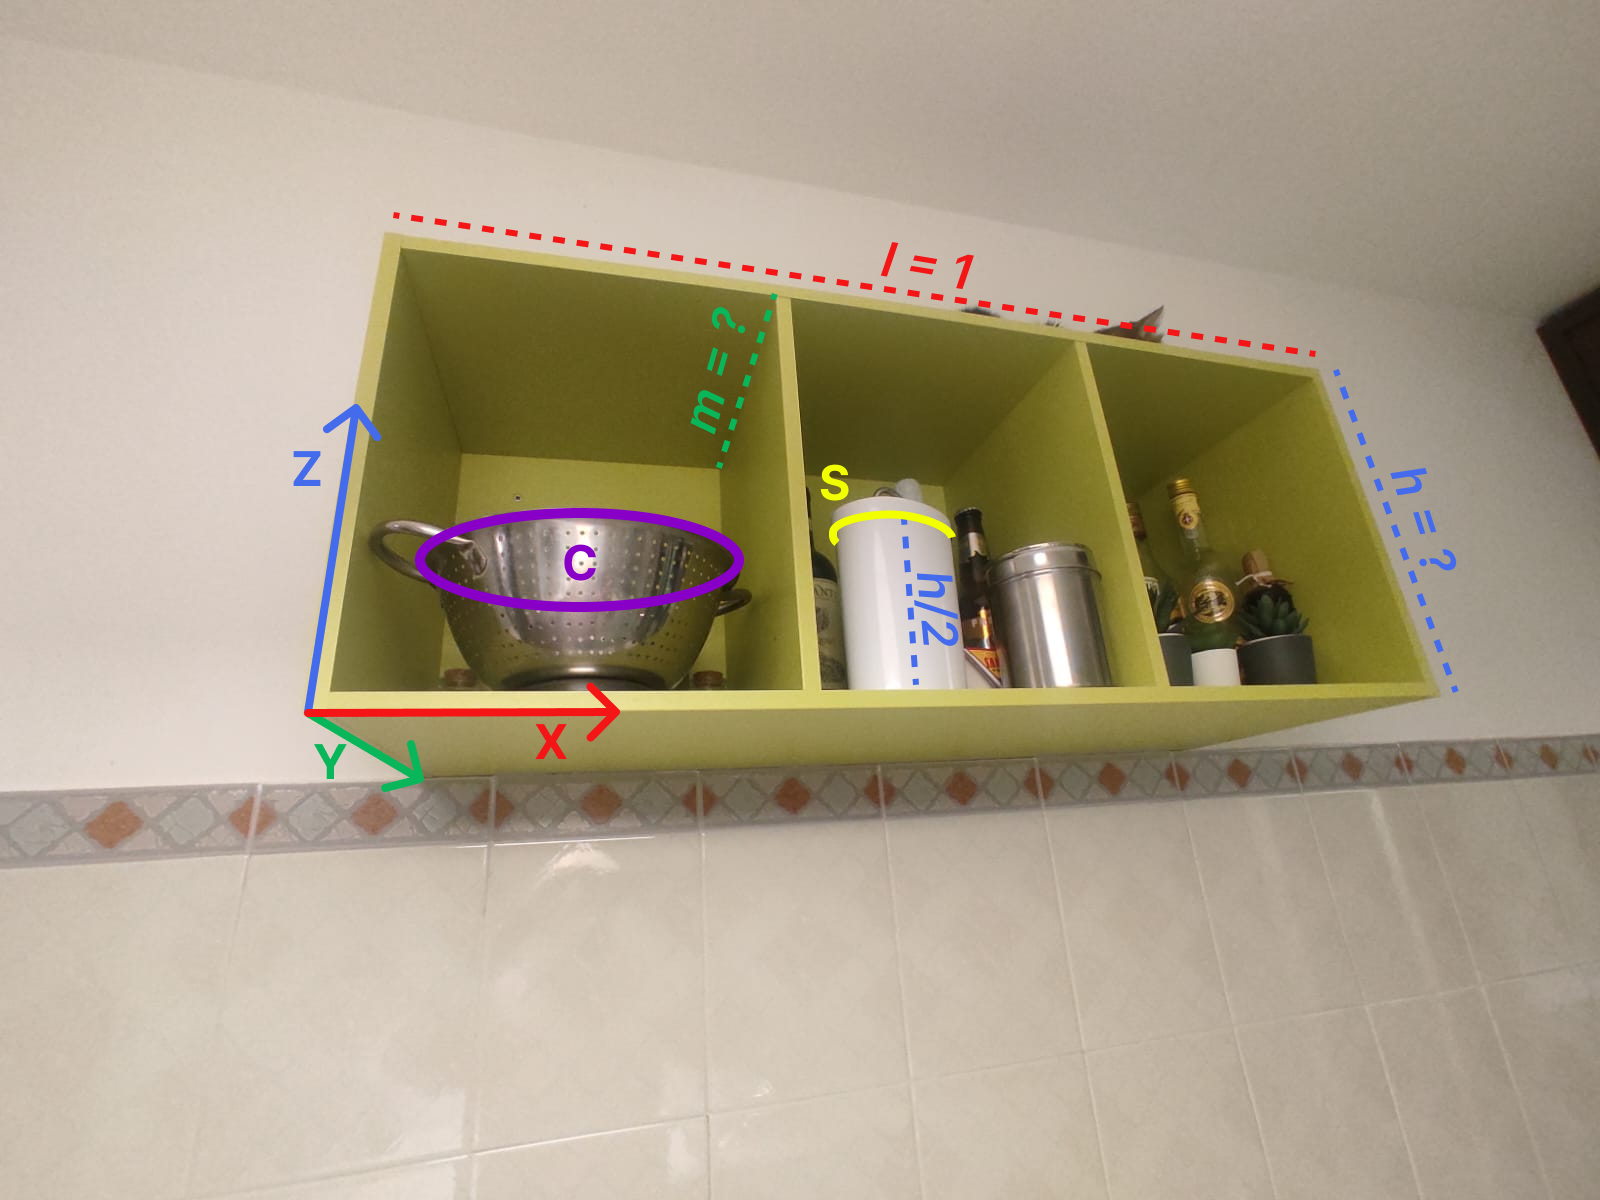
\includegraphics[height=9.5cm, width=\textwidth, keepaspectratio]{Report/Images/Introduction/Scene Description.png}
\caption{\label{fig:SceneDescription}The Scene Description}
\end{figure}

\subsection{Image Description}
A single image is taken of the above rectangular parallelepiped by an uncalibrated, zero
skew, camera. (Its calibration matrix $K$ depends on four unknown parameters, namely $f_x$, $f_y$ and 
the two pixel coordinates $U_O$, $V_O$ of the principal point). A set of lines parallel to X-axis are visible, and their images $l_1$, $l_2$ and $l_3$ are extracted; a set of lines parallel to the $Y$-axis are visible and their images  $m_1$, $m_2$, $m_3$, $m_4$, $m_5$ and $m_6$ are extracted; a set of vertical lines (i.e., parallel to the $Z$
axis) are also visible and their images $h_1$, $h_2$, $h_3$ and $h_4$ are extracted.  In addition, both the image $C$ of the circumference and the image $S$ of the unknown horizontal curve are also extracted.  


\label{ch:introduction}

\chapter{Feature Extraction}
\label{ch:Feature Extraction}

\section{Conic Extraction}
In order to extract the conic $C$:
\begin{enumerate}
    \item Crop the image to the desired portion
    \begin{figure}[H]
    \centering
    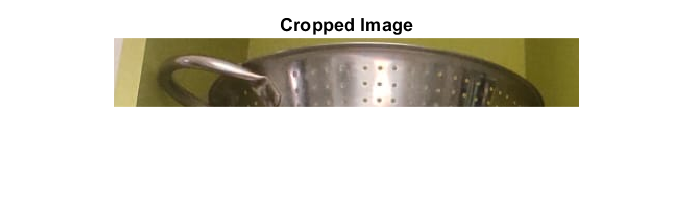
\includegraphics[height=9.5cm, width=\textwidth, keepaspectratio]{Report/Images/Features/Conic/CroppedImage.png}
    \caption{\label{fig:conic:cropped image}The image cropped}
    \end{figure}

    \item Convert to gray scale
    \begin{figure}[H]
    \centering
    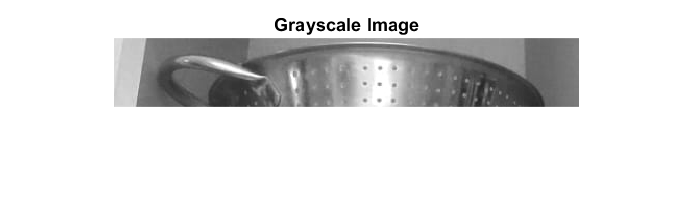
\includegraphics[height=9.5cm, width=\textwidth, keepaspectratio]{Report/Images/Features/Conic/GrayscaleImage.png}
    \caption{\label{fig:conic:gray scale}The image in grey scale}
    \end{figure}

    \item Canny edge detection ($\sigma = 2$, threshold = $[0, 0.15]$)
        \begin{figure}[H]
    \centering
    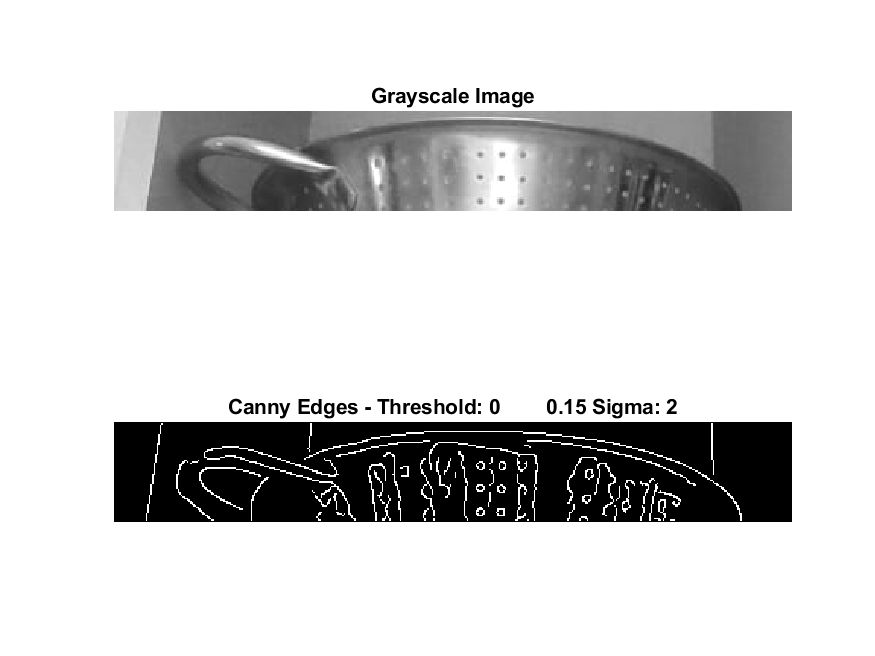
\includegraphics[height=9.5cm, width=\textwidth, keepaspectratio]{Report/Images/Features/Conic/CannyEdges.png}
    \caption{\label{fig:conic:edges}Canny Edge detection}
    \end{figure}

    \item Remove edges that are too crowded, like the holes of the colander. To do that, first heavily blur the image ($\sigma = 10$) then threshold the image to select the sparser areas ($\leq 0.1$). Use this to mask the edges
            \begin{figure}[H]
    \centering
    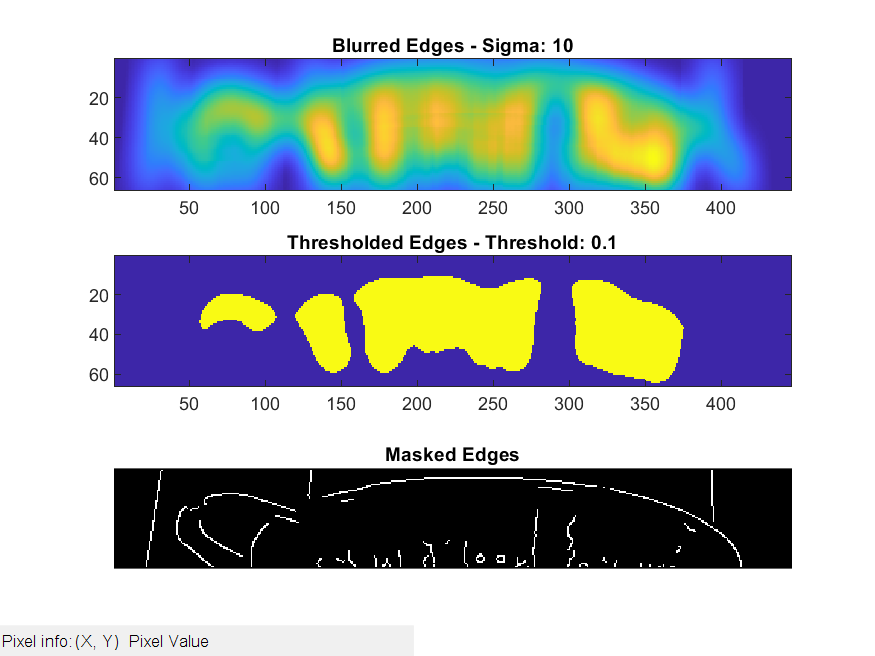
\includegraphics[height=9.5cm, width=\textwidth, keepaspectratio]{Report/Images/Features/Conic/MaskedEdges.png}
    \caption{\label{fig:conic:mask}Masking the edges}
    \end{figure}

    \item Extract the remaining points $\neq 0$ and use a slightly modified RANSAC to extract the Conic with the most inliers 
                \begin{figure}[H]
    \centering
    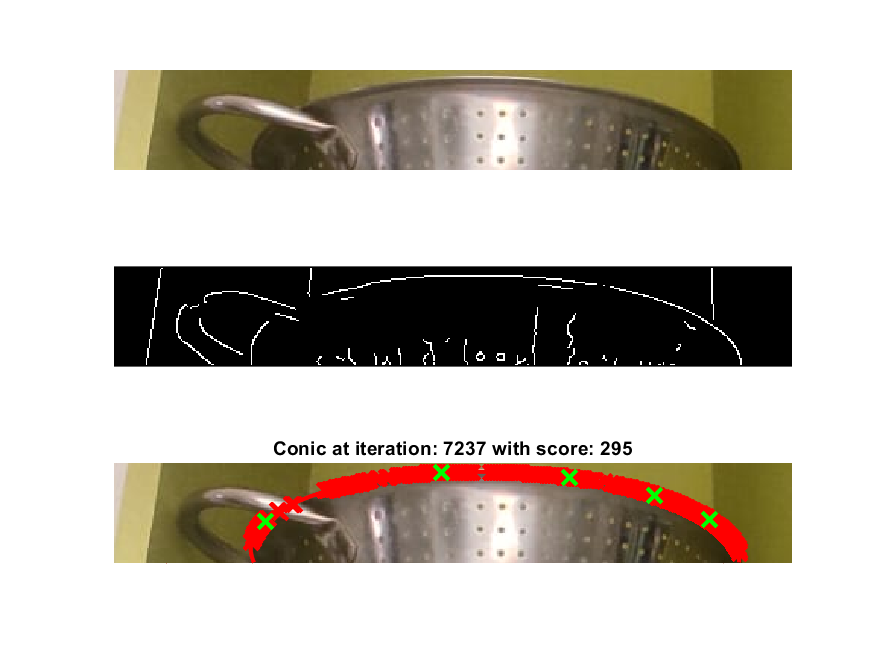
\includegraphics[height=9.5cm, width=\textwidth, keepaspectratio]{Report/Images/Features/Conic/ConicRANSAC.png}
    \caption{\label{fig:conic:ransac}Conic RANSAC}
    \end{figure}

                    \begin{figure}[H]
    \centering
    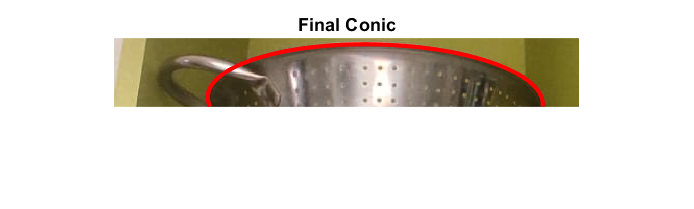
\includegraphics[height=9.5cm, width=\textwidth, keepaspectratio]{Report/Images/Features/Conic/FinalConic.png}
    \caption{\label{fig:conic:final}Final Conic}
    \end{figure}

    
\end{enumerate}

\section{Extraction of $S$ curve}

In order to extract the curve $S$:
\begin{enumerate}
    \item Crop the image to the desired portion
    \item Convert to grayscale
    \item Canny edge detection ($\sigma = 1$, threshold = $[0.2, 0.8]$)
\end{enumerate}
\chapter{Scene Geometry Reconstruction}
\label{ch:Scene Geometry}

\section{Finding the vanishing line $l'_\infty$ of the horizontal plane}

\begin{Procedure}[label=proc:FindingIntersection]{Robust finding of the intersection between multiple intersecting lines}
This procedure aims at finding the intersection point $P$ of a given set of $n \geq 2$ intersecting lines $l_i \, \forall i \in \{1, ..., n\}$. Both the point $P$ and the lines $l_i$ are provided in homogenous coordinates. Thus $$\underline{P} \overset{\Delta}{=} \colvec{P_x, P_y, 1}$$ and $$\underline{l_i} \overset{\Delta}{=} \colvec{l_{ix}, l_{iy}, 1} \, \forall i \in \{1, ..., n\}$$. The matrix $L$ is defined as $$L = \matrixdim{1}{4}{\underline{l_1}, \underline{l_2}, \dots, \underline{l_n}}$$

Were all the lines perfectly intersecting in a single point it would hold $$L^T\underline{P} = \underline{0}$$

and thus

$$\underline{P} \in RNS(L)$$

Unfortunately, in the real world, seldom do $n$ "intersecting" lines actually intersect. An approximated solution is needed and thus the problem becomes an optimization one:

$$
\underline{P} \overset{\Delta}{=} \argmin_{\underline{x}} ||L^T\underline{x}||_2
$$

This problem can be solved using the Singular Value Decomposition (SVD) on the $L$ matrix:
\begin{equation}
    \begin{matrix}
        L = U \Sigma V^T \\
        \text{ where } \\
        U, \Sigma, V \in \mathbb{R}^{3x3}, \\
        U\cdot U^T = I, \\
        V\cdot V^T = I,\\
        \Sigma_{ii} = \sigma_i \in \mathbb{R} \; \forall i \in \{1, ..., 3\}, \\
         \Sigma_{ij} = 0 \; \forall i \in \{1, ..., 3\}, \forall j \in \{1, ..., 3\}, i\neq j, \\
         |\sigma_i| >= |\sigma_j| \; \forall i, j \in \{1, ..., 3\}, i<j
    \end{matrix}
\end{equation}

Since the $\sigma_i$ are in absolute nonincreasing order it can be easily derived that the optimal solution up to scale is:

$$
\underline{P} \overset{\Delta}{=} V_n := \text{n-th column of V}
$$
\end{Procedure}

The image of the vanishing line $l'_\infty$ of the horizontal plane can be found as the line going through the images of two distinct vanishing points of the horizontal plane. Luckily, the vanishing point associated with a direction in the horizontal plane is shared with all parallel planes, and thus the $m$s and $l$s lines will all meet respectively in the vanishing points $v_m$ and $v_l$. 

Using Procedure~\ref{proc:FindingIntersection} the best approximation for $v_m$ and $v_l$ can be computed.

The line $l'_\infty$ is now defined as :

\begin{equation*}
\begin{split}
l'_{\infty{}}^T v_m &= 0\\
l'_{\infty{}}^T v_l &= 0
\end{split}
\end{equation*}

and thus:

$$
l'_\infty{} \overset{\Delta}{=} v_m \times v_l
$$

The results of the extraction are the following:

$$
l'_\infty{} \overset{\Delta}{=}\colvec{-8.0288 \cdot 10^{-05}, -0.0011, 1}
$$

\begin{figure}[H]
\centering
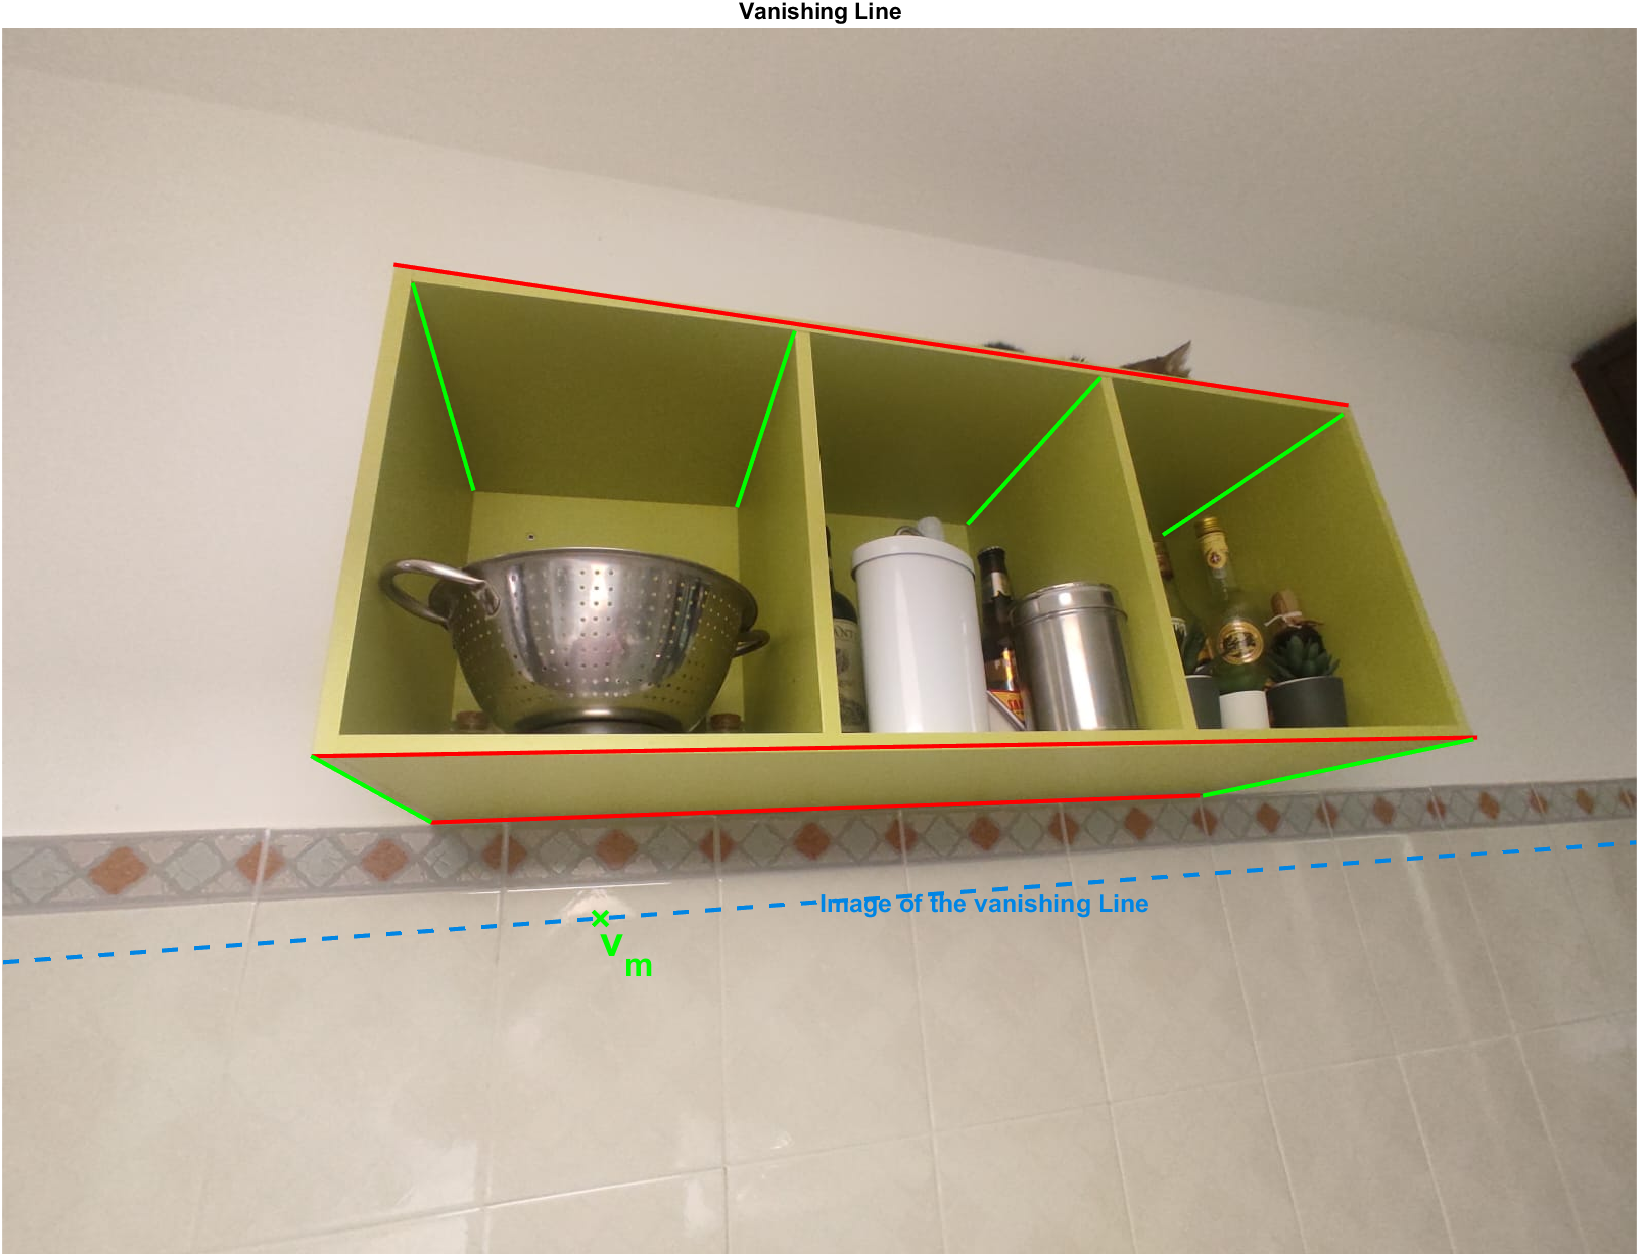
\includegraphics[height=9.5cm, width=\textwidth, keepaspectratio]{Report/Images/2.1-VanishingLine/Vanishing Line.png}
\caption{\label{fig:Vanishing Line}The Extracted image of the vanishing line}
\end{figure}


\section{Metric Rectification and depth estimation}
To rectify the upper face of the cabinet a stratified approach has been chosen. The rectification is the outcome of three steps:
\begin{enumerate}
    \item Affine Rectification
    \item Affinity to make $C$ a circle
    \item Affinity to align the axis and allign the plot (optional)
\end{enumerate}

\subsection{Affine Rectification}
The purpose of the affine rectification is to find the Homography $H_{aff}$ such that $$H_{aff}^{-T} 
 \cdot l_{\infty{}}' = l_\infty{} = \colvec{0, 0, 1}$$

 Consequently $H_{aff}$ has to be of this form:
 $$
 H_{aff} = \matrixdim{3}{3}{*, *, *, *, *, *, ,l_{\infty{}}'^T, }
 $$

 In order to make the affine reconstructed image of a more manageable size the following homography has been chosen:

  $$
 H_{aff} = \matrixdim{3}{3}{\frac{1}{10}, 0, 0, 0, \frac{1}{10}, 0,-8.0288 \cdot 10^{-05}, -0.0011, 1}
 $$

 \begin{figure}[H]
\centering
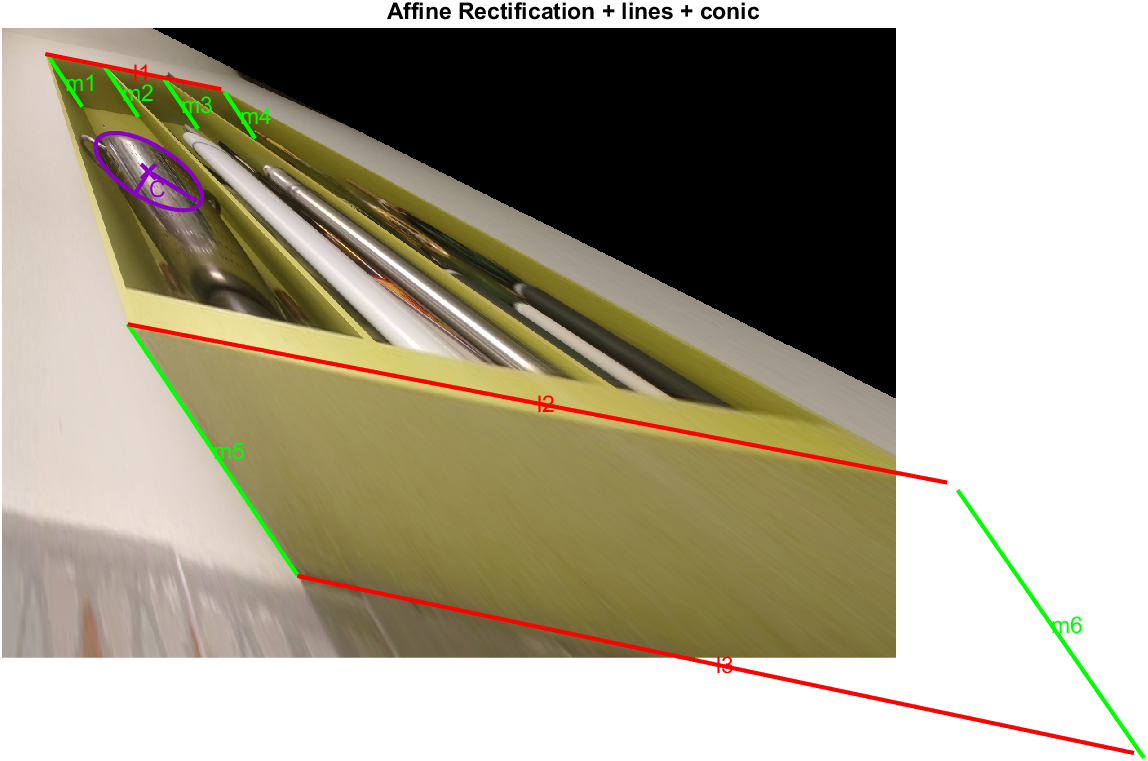
\includegraphics[height=9.5cm, width=\textwidth, keepaspectratio]{Report/Images/2.2-MetricRectification/Affine Rectification.png}
\caption{\label{fig:Affine rectification}The result of the affine rectification}
\end{figure}

\subsection{Affinity to make $C$ a circle}
Given the extracted conic $C$ in homogeneous matrix form, one can apply the affine rectification obtaining:
$$
C_{aff} = H_{aff}^{-T} \cdot C \cdot H_{aff}^{-1}
$$

From that the length ($a$ and $b$) and direction ($\theta$) of the ellipse' axis as well as the ellipse center's coordinates ($C_c$) can be extracted:

\begin{equation*}
\begin{split}
a &= 74.0106\text{ pixels}\\
b &= 31.8570\text{ pixels}\\
\theta &= 0.5529\text{ rad}\\
C_C &= \colvec{180.4210, 176.4675, 1} \text{ pixels}
\end{split}
\end{equation*}

The Homography necessary to turn $C_{aff}$ back into a circle can be factored into an isometry $U$ and a scaling $S$ as $H_{circle} = U S U^{-1}$. The two homographies can be built as follows:

\begin{equation*}
\begin{split}
U &= \matrixdim{3}{3}{\cos{\theta}, -\sin{\theta}, , \sin{\theta}, \cos{\theta}, C_c, 0, 0, }\\
S &= \matrixdim{3}{3}{1, 0, 0, 0, a/b, 0, 0, 0, 1}\\
\theta &= 0.5529\text{ rad}
\end{split}
\end{equation*}

Thus a shape reconstructing homography can be:
$$H_{metric} = H_{circle} \cdot H_{aff}$$

\subsection{Affinity to align the axis and align the plot (optional)}

To facilitate subsequent tasks another affinity is necessary to align the $l$ lines to the x-axis and to center the plot. This is encapsulated in $H_{offset}$

The final Rectifing Homography is thus:

$$H_{metric} = H_{off} \cdot H_{circle} \cdot H_{aff} = \matrixdim{3}{3}{0.1041, -0.2222, 138.2097, -0.0286, 0.1633, -14.5239, -0.0001, -0.0011, 1}$$

The result of the rectification is the following:

\begin{figure}[H]
\centering
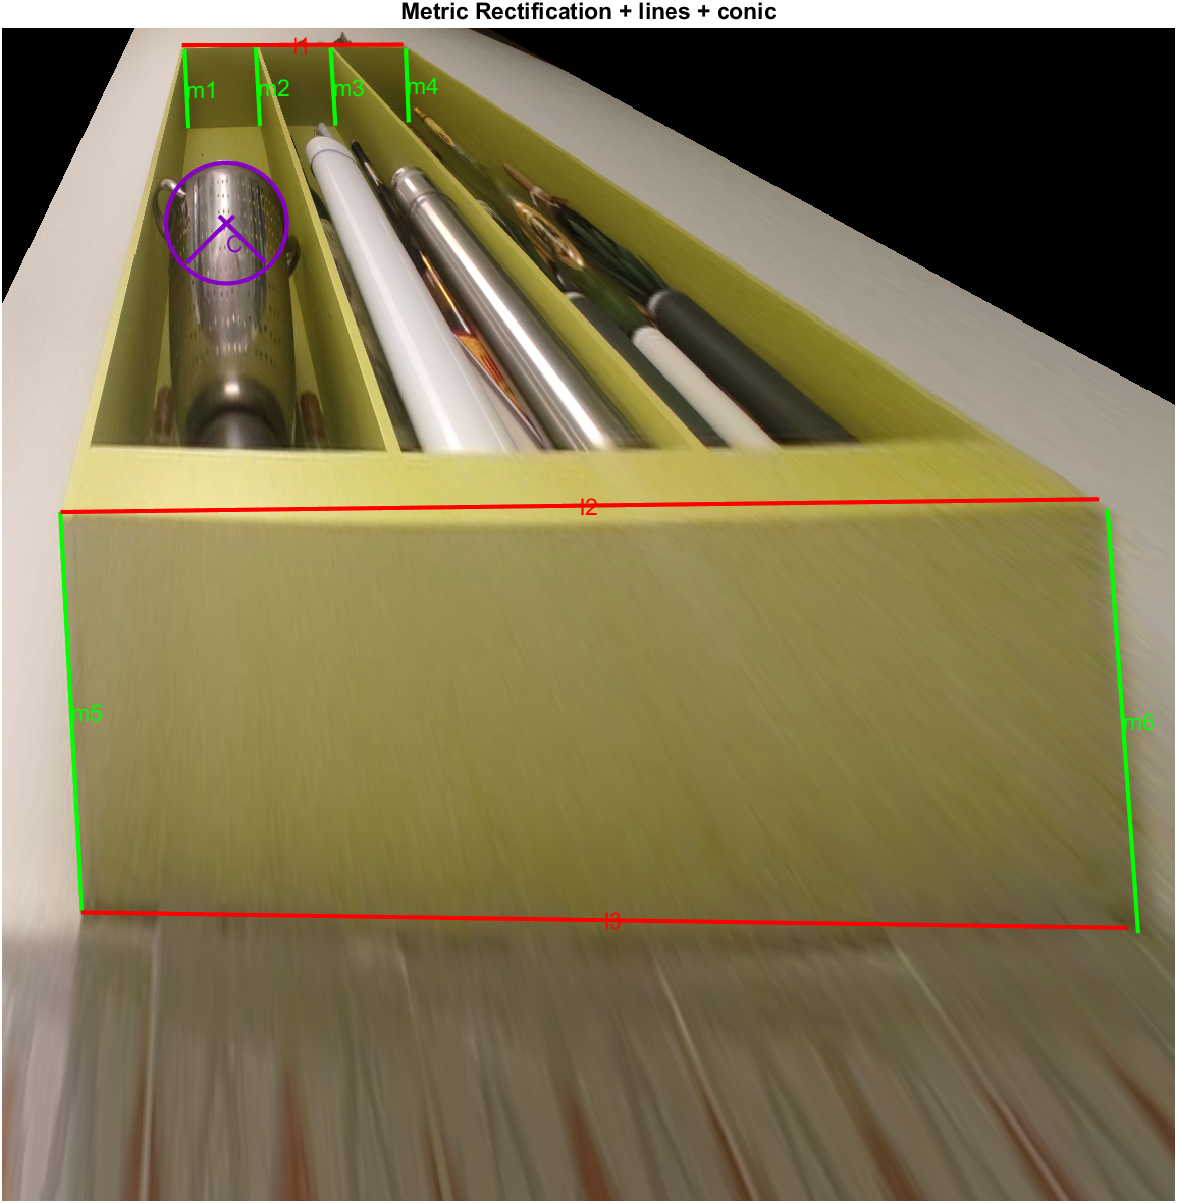
\includegraphics[height=9.5cm, width=\textwidth, keepaspectratio]{Report/Images/2.2-MetricRectification/Metric Rectification.png}
\caption{\label{fig:Metric rectification}The result of the metric rectification}
\end{figure}

\subsection{Depth estimation}
Estimating the depth $m$ is only a matter of measuring the right things. $m_5$ and $m_6$ are the only lines spanning the whole depth and they are both coplanar to $l_2$ and $l_3$ that are both 1 unit long in the scene. Since lines that share the same horizontal plane have the same scaling factor in the metric rectification, follows that by calling $m_{5_1}^m$, $m_{5_2}^m$, $m_{6_1}^m$, $m_{6_2}^m$ $l_{2_1}^m$, $l_{2_2}^m$, $l_{3_1}^m$, $l_{3_2}^m$ the homogenous coordinates of the pixel coordinated of the endpoints of the segments in the metric rectified image, the depth is:

$$
m = \frac{||m_{5_1}^m - m_{5_2}^m|| + ||m_{6_1}^m - m_{6_2}^m||}{||l_{2_1}^m - l_{2_2}^m|| + ||l_{3_1}^m - l_{3_2}^m||} = 0.39571 \text{ units} 
$$

With the exact same reasoning translated to the $m_{1:4}$ and $l_1$ lines, the internal depth of the cabinet can be computed:

$$
m_{internal} = 0.35073 \text{ units} 
$$

With this two information, the depth of the back plate of the cabinet can be estimated (This will come in handy for the 3D model reconstruction).

$$
m_{backplate} = m - m_{internal} = 0.044985 \text{ units}
$$

\section{Intrinsic Calibration}
The goal of this task is to find the calibration matrix $K$ built as follows:
$$
K = \matrixdim{3}{3}{f_x, 0, U_0, 0, f_y, V_0, 0, 0, 1}
$$

Instead of estimating $K$ directly, it is easier to find $\omega \overset{\Delta}{=} (KK^T)^{-1}$.
This matrix is built as follows:
$$
\omega = \matrixdim{3}{3}{a^2, 0, -U_0a^2, 0, 1, -V_0, -U_0a^2, -V_0, f_y^2+a^2U_0^2+V_0^2}
$$


By knowing an homography $H = [h_1, h_2, h_3]$ that goes from the coordinate on a plane $\pi$ to the image space and the vanishing point $v$ along the direction orthogonal to $\pi$, the following conditions must hold:
\begin{equation*}
\begin{split}
h_1^T\omega h_2 &= 0 \\
h_1^T\omega h_1 - h_2^T\omega h_2 &= 0\\
v^T\omega h_1 &= 0 \\
v^T\omega h_2 &= 0
\end{split}
\end{equation*}

And thus the entries of $\omega$ can be estimated as solutions of a linear system of equations.

$K$ can then be reconstructed with the Cholesky decomposition of $\omega^-1$.

In this case, the homography $H$ used is equal to $H_{metric}^{-1}$ thus setting the plane $\pi$ to be horizontal. The vanishing point $v$ can be computed with Procedure~\ref{proc:FindingIntersection} on the lines $h_{1:4}$.

The estimated calibration matrix is:
$$
K = \matrixdim{3}{3}{782.3411, 0, 800.8240, 0, 789.2100, 534.6531, 0, 0, 1}
$$

\section{Height estimation}
By multiplying $H$ with $K^{-1}$, a set of basis of $\pi$ $r1$ and $r2$ and the offset $o_\pi$ are obtained, expressed in the reference frame of the camera:
$$\matrixdim{1}{3}{r_1, r_2, o_\pi} = K^{-1}H$$

These coordinates are known up to scale, which is the key for selecting planes at a given height. That's because it is known that the segments $l_{1:3}$ are 1 unit long in the scene, thus by dividing the vectors by the length of the metric rectified  $l_1^m$ ($|l_1^m|$) or $l_2^m$ ($|l_2^m|$), a set of 3D origin and coordinates of the upper and lower face of the cabinet can be found. Calling $\hat{r_3}$ a unit vector orthogonal to both $r_1$ and $r_2$, the height can be simply computed as:
$$
h = \hat{r_3}^T \cdot (\frac{o_\pi}{|l_1^m|} - \frac{o_\pi}{|l_2^m|}) = (\frac{1}{|l_1^m|} - \frac{1}{|l_2^m|}) \hat{r_3}^T \cdot o_\pi = 0.3842 \text{ units}
$$




\chapter*{Introduction}

This document is intended to be both an example of the Polimi \LaTeX{} template for Master Theses,
as well as a short introduction to its use. It is not intended to be a general introduction to \LaTeX{} itself,
and the reader is assumed to be familiar with the basics of creating and compiling \LaTeX{} documents (see \cite{oetiker1995not, kottwitz2015latex}). 
\\
The cover page of the thesis must contain all the relevant information:
title of the thesis, name of the Study Programme and School, name of the author,
student ID number, name of the supervisor, name(s) of the co-supervisor(s) (if any), academic year.
The above information are provided by filling all the entries in the command \verb|\puttitle{}|
in the title page section of this template.
\\
Be sure to select a title that is meaningful.
It should contain important keywords to be identified by indexer.
Keep the title as concise as possible and comprehensible even to people who are not experts in your field.
The title has to be chosen at the end of your work so that it accurately captures the main subject of the manuscript. 
\\
Since a thesis might be a substantial document, it is convenient to break it into chapters.
You can create a new chapter as done in this template by simply using the following command
\begin{verbatim}
\chapter{Title of the chapter}
\end{verbatim}
followed by the body text.
\\
Especially for long manuscripts, it is recommended to give each chapter its own file.
In this case, you write your chapter in a separated \verb|chapter_n.tex| file
and then include it in the main file with the following command
\begin{verbatim}
\input{chapter_n.tex}
\end{verbatim}
It is recommended to give a label to each chapter by using the command
\begin{verbatim}
\label{ch:chapter_name}%
\end{verbatim}
where the argument is just a text string that you'll use to reference that part
as follows: \textit{Chapter~\ref{ch:chapter_one} contains \sc{an introduction to}  \dots}.\\
If necessary, an unnumbered chapter can be created by
\begin{verbatim}
\chapter*{Title of the unnumbered chapter}
\end{verbatim}
\label{ch:intro_tamplate}

% Import of Chapter One from the template
\chapter{Chapter one}
\label{ch:chapter_one}%
% The \label{...}% enables to remove the small indentation that is generated, always leave the % symbol.

In this chapter additional useful information are reported.

\section{Sections and subsections}
\label{sec:section_name}
Chapters are typically subdivided into sections and subsections, and, optionally,
subsubsections, paragraphs and subparagraphs.
All can have a title, but only sections and subsections are numbered.
A new section is created by the command
\begin{verbatim}
\section{Title of the section}
\end{verbatim}
The numbering can be turned off by using \verb|\section*{}|.
\\
A new subsection is created by the command
\begin{verbatim}
\subsection{Title of the subsection}
\end{verbatim}
and, similarly, the numbering can be turned off by adding an asterisk as follows 
\begin{verbatim}
\subsection*{}
\end{verbatim}

\section{Equations}
\label{sec:eqs}
This section gives some examples of writing mathematical equations in your thesis.

Maxwell's equations read:
\begin{subequations}
    \label{eq:maxwell}
    \begin{align}[left=\empheqlbrace]
    \nabla\cdot \bm{D} & = \rho, \label{eq:maxwell1} \\
    \nabla \times \bm{E} +  \frac{\partial \bm{B}}{\partial t} & = \bm{0}, \label{eq:maxwell2} \\
    \nabla\cdot \bm{B} & = 0, \label{eq:maxwell3} \\
    \nabla \times \bm{H} - \frac{\partial \bm{D}}{\partial t} &= \bm{J}. \label{eq:maxwell4}
    \end{align}
\end{subequations}

Equation~\eqref{eq:maxwell} is automatically labeled by \texttt{cleveref},
as well as Equation~\eqref{eq:maxwell1} and Equation~\eqref{eq:maxwell3}.
Thanks to the \verb|cleveref| package, there is no need to use \verb|\eqref|.
Remember that Equations have to be numbered only if they are referenced in the text.

Equations~\eqref{eq:maxwell_multilabels1}, \eqref{eq:maxwell_multilabels2}, \eqref{eq:maxwell_multilabels3}, and \eqref{eq:maxwell_multilabels4} show again Maxwell's equations without brace:
\begin{align}
    \nabla\cdot \bm{D} & = \rho, \label{eq:maxwell_multilabels1} \\
    \nabla \times \bm{E} +  \frac{\partial \bm{B}}{\partial t} &= \bm{0}, \label{eq:maxwell_multilabels2} \\
    \nabla\cdot \bm{B} & = 0, \label{eq:maxwell_multilabels3} \\
    \nabla \times \bm{H} - \frac{\partial \bm{D}}{\partial t} &= \bm{J} \label{eq:maxwell_multilabels4}.
\end{align}

Equation~\eqref{eq:maxwell_singlelabel} is the same as before,
but with just one label:
\begin{equation}
    \label{eq:maxwell_singlelabel}
    \left\{
    \begin{aligned}
    \nabla\cdot \bm{D} & = \rho, \\
    \nabla \times \bm{E} +  \frac{\partial \bm{B}}{\partial t} &= \bm{0},\\
    \nabla\cdot \bm{B} & = 0, \\
    \nabla \times \bm{H} - \frac{\partial \bm{D}}{\partial t} &= \bm{J}.
    \end{aligned}
    \right.
\end{equation}

\section{Figures, Tables and Algorithms}
Figures, Tables and Algorithms have to contain a Caption that describe their content, and have to be properly reffered in the text.

\subsection{Figures}
\label{subsec:figures}

For including pictures in your text you can use \texttt{TikZ} for high-quality hand-made figures,
or just include them as usual with the command
\begin{verbatim}
\includegraphics[options]{filename.xxx}
\end{verbatim}
Here xxx is the correct format, e.g. \verb|.png|, \verb|.jpg|, \verb|.eps|, \dots.

\begin{figure}[H]
    \centering
    
\includegraphics[width=0.3\textwidth]{logo_polimi_scritta.eps}
    \caption{Caption of the Figure to appear in the List of Figures.}
    \label{fig:quadtree}
\end{figure}

Thanks to the \texttt{\textbackslash subfloat} command, a single figure, such as Figure~\ref{fig:quadtree},
can contain multiple sub-figures with their own caption and label, e.g. \color{black} Figure~\ref{fig:polimi_logo1} and Figure~\ref{fig:polimi_logo2}. 

\begin{figure}[H]
    \centering
    \subfloat[One PoliMi logo.\label{fig:polimi_logo1}]{
        
\includegraphics[scale=0.5]{Images/logo_polimi_scritta.eps}
    }
    \quad
    \subfloat[Another one PoliMi logo.\label{fig:polimi_logo2}]{
        
\includegraphics[scale=0.5]{Images/logo_polimi_scritta2.eps}
    }
    \caption[Shorter caption]{This is a very long caption you don't want to appear in the List of Figures.}
    \label{fig:quadtree2}
\end{figure}


\subsection{Tables}
\label{subsec:tables}

Within the environments \texttt{table} and  \texttt{tabular} you can create very fancy tables as the one shown in Table~\ref{table:example}.
\begin{table}[H]
    \caption*{\textbf{Title of Table (optional)}}
    \centering 
    \begin{tabular}{|p{3em} c c c |}
    \hline
    \rowcolor{bluepoli!40} % comment this line to remove the color
     & \textbf{column 1} & \textbf{column 2} & \textbf{column 3} \T\B \\
    \hline \hline
    \textbf{row 1} & 1 & 2 & 3 \T\B \\
    \textbf{row 2} & $\alpha$ & $\beta$ & $\gamma$ \T\B\\
    \textbf{row 3} & alpha & beta & gamma \B\\
    \hline
    \end{tabular}
    \\[10pt]
    \caption{Caption of the Table to appear in the List of Tables.}
    \label{table:example}
\end{table}

You can also consider to highlight selected columns or rows in order to make tables more readable.
Moreover, with the use of \texttt{table*} and the option \texttt{bp} it is possible to align them at the bottom of the page. One example is presented in Table~\ref{table:exampleC}. 

\begin{table}[H]
\centering 
    \begin{tabular}{|p{3em} | c | c | c | c | c | c|}
    \hline
%    \rowcolor{bluepoli!40}
     & \textbf{column1} & \textbf{column2} & \textbf{column3} & \textbf{column4} & \textbf{column5} & \textbf{column6} \T\B \\
    \hline \hline
    \textbf{row1} & 1 & 2 & 3 & 4 & 5 & 6 \T\B\\
    \textbf{row2} & a & b & c & d & e & f \T\B\\
    \textbf{row3} & $\alpha$ & $\beta$ & $\gamma$ & $\delta$ & $\phi$ & $\omega$ \T\B\\
    \textbf{row4} & alpha & beta & gamma & delta & phi & omega \B\\
    \hline
    \end{tabular}
    \\[10pt]
    \caption{Highlighting the columns}
    \label{table:exampleC}
\end{table}

\begin{table}[H]
\centering 
    \begin{tabular}{|p{3em} c c c c c c|}
    \hline
%    \rowcolor{bluepoli!40}
     & \textbf{column1} & \textbf{column2} & \textbf{column3} & \textbf{column4} & \textbf{column5} & \textbf{column6} \T\B \\
    \hline \hline
    \textbf{row1} & 1 & 2 & 3 & 4 & 5 & 6 \T\B\\
    \hline
    \textbf{row2} & a & b & c & d & e & f \T\B\\
    \hline
    \textbf{row3} & $\alpha$ & $\beta$ & $\gamma$ & $\delta$ & $\phi$ & $\omega$ \T\B\\
    \hline
    \textbf{row4} & alpha & beta & gamma & delta & phi & omega \B\\
    \hline
    \end{tabular}
    \\[10pt]
    \caption{Highlighting the rows}
    \label{table:exampleR}
\end{table}

\subsection{Algorithms}
\label{subsec:algorithms}

Pseudo-algorithms can be written in \LaTeX{} with the \texttt{algorithm} and \texttt{algorithmic} packages.
An example is shown in Algorithm~\ref{alg:var}.
\begin{algorithm}[H]
    \label{alg:example}
    \caption{Name of the Algorithm}
    \label{alg:var}
    \label{protocol1}
    \begin{algorithmic}[1]
    \STATE Initial instructions
    \FOR{$for-condition$}
    \STATE{Some instructions}
    \IF{$if-condition$}
    \STATE{Some other instructions}
    \ENDIF
    \ENDFOR
    \WHILE{$while-condition$}
    \STATE{Some further instructions}
    \ENDWHILE
    \STATE Final instructions
    \end{algorithmic}
\end{algorithm} 

\vspace{5mm}

\section{Theorems, propositions and lists}

\subsection{Theorems}
Theorems have to be formatted as:
\begin{theorem}
\label{a_theorem}
Write here your theorem. 
\end{theorem}
\textit{Proof.} If useful you can report here the proof.

\subsection{Propositions}
Propositions have to be formatted as:
\begin{proposition}
Write here your proposition.
\end{proposition}

\subsection{Lists}
How to  insert itemized lists:
\begin{itemize}
    \item first item;
    \item second item.
\end{itemize}
How to insert numbered lists:
\begin{enumerate}
    \item first item;
    \item second item.
\end{enumerate}

\section{Use of copyrighted material}

Each student is responsible for obtaining copyright permissions, if necessary, to include published material in the thesis.
This applies typically to third-party material published by someone else.

\section{Plagiarism}

You have to be sure to respect the rules on Copyright and avoid an involuntary plagiarism.
It is allowed to take other persons' ideas only if the author and his original work are clearly mentioned.
As stated in the Code of Ethics and Conduct, Politecnico di Milano \textit{promotes the integrity of research,
condemns manipulation and the infringement of intellectual property}, and gives opportunity to all those
who carry out research activities to have an adequate training on ethical conduct and integrity while doing research.
To be sure to respect the copyright rules, read the guides on Copyright legislation and citation styles available
at:
\begin{verbatim}
https://www.biblio.polimi.it/en/tools/courses-and-tutorials
\end{verbatim}
You can also attend the courses which are periodically organized on "Bibliographic citations and bibliography management".

\section{Bibliography and citations}
Your thesis must contain a suitable Bibliography which lists all the sources consulted on developing the work.
The list of references is placed at the end of the manuscript after the chapter containing the conclusions.
We suggest to use the BibTeX package and save the bibliographic references  in the file \verb|Thesis_bibliography.bib|.
This is indeed a database containing all the information about the references. To cite in your manuscript, use the \verb|\cite{}| command as follows:
\\
\textit{Here is how you cite bibliography entries: \cite{knuth74}, or multiple ones at once: \cite{knuth92,lamport94}}.
\\
The bibliography and list of references are generated automatically by running BibTeX \cite{bibtex}.
\label{ch:tamplate}%

\chapter{Conclusions and future developments}
\label{ch:conclusions}%
A final chapter containing the main conclusions of your research/study
and possible future developments of your work have to be inserted in this chapter.

%-------------------------------------------------------------------------
%	BIBLIOGRAPHY
%-------------------------------------------------------------------------

\addtocontents{toc}{\vspace{2em}} % Add a gap in the Contents, for aesthetics
\bibliography{Thesis_bibliography} % The references information are stored in the file named "Thesis_bibliography.bib"

%-------------------------------------------------------------------------
%	APPENDICES
%-------------------------------------------------------------------------

\cleardoublepage
\addtocontents{toc}{\vspace{2em}} % Add a gap in the Contents, for aesthetics
\appendix
\chapter{Appendix A}
If you need to include an appendix to support the research in your thesis, you can place it at the end of the manuscript.
An appendix contains supplementary material (figures, tables, data, codes, mathematical proofs, surveys, \dots)
which supplement the main results contained in the previous chapters.

\chapter{Appendix B}
It may be necessary to include another appendix to better organize the presentation of supplementary material.


% LIST OF FIGURES
\listoffigures

% LIST OF TABLES
\listoftables

% LIST OF SYMBOLS
% Write out the List of Symbols in this page
\chapter*{List of Symbols} % You have to include a chapter for your list of symbols (
\begin{table}[H]
    \centering
    \begin{tabular}{lll}
        \textbf{Variable} & \textbf{Description} & \textbf{SI unit} \\\hline\\[-9px]
        $\bm{u}$ & solid displacement & m \\[2px]
        $\bm{u}_f$ & fluid displacement & m \\[2px]
    \end{tabular}
\end{table}

% ACKNOWLEDGEMENTS
\chapter*{Acknowledgements}
Here you might want to acknowledge someone.

\cleardoublepage

\end{document}
